\documentclass[10pt,twocolumn,letterpaper]{article}

% =====================================================================
% CVPR/ICCV submission template (drafting preamble; swap in the official
% cvpr.sty for camera-ready).
% =====================================================================

\usepackage[margin=0.9in]{geometry}
\usepackage{graphicx}
\usepackage{amsmath,amssymb}
\usepackage{booktabs}
\usepackage{multirow}
\usepackage{xcolor}
\usepackage[colorlinks=true,allcolors=blue]{hyperref}
\usepackage{caption}
\usepackage{subcaption}

\graphicspath{{figs/}}
\renewcommand{\ttdefault}{cmtt}

\newcommand{\method}{\textsc{Fusion-Splat}}

\title{Distance-Adaptive Generative Supervision for\\
Feed-Forward Single-View 3D Gaussian Splatting}
\author{Anonymous submission\\\small Paper ID ****}
\date{}

\begin{document}
\maketitle

\begin{abstract}
Feed-forward single-view 3D Gaussian Splatting (e.g., Flash3D) reconstructs a
scene from one image in a single forward pass, but its novel-view renders
degrade at large viewpoint changes with stretching, ghosting and blur. We study
using a \emph{generative image prior} to supervise a short per-scene
optimization that repairs these renders back into the 3D representation, and we
make a key observation: two kinds of generative supervisor have complementary
strengths. A single-step image restorer (Difix) improves perceptual quality
(LPIPS/FID) but not pixel accuracy, whereas a video-diffusion generator
(ViewCrafter) recovers pixel accuracy (PSNR) at large baselines but drifts in
color/texture and hurts LPIPS. We show these are two ends of a trade-off and
propose \method{}, a \emph{distance-adaptive fusion} that supervises near views
with the image restorer and blends toward the video generator as the viewpoint
departs from the input. On the RealEstate10K MINE single-view protocol (standard
$256{\times}384$), \method{} is the only method that improves \emph{every}
metric at \emph{every} baseline over Flash3D: at large viewpoints it gains
$+0.03$\,dB PSNR (vs.\ $-0.09$ for the image restorer alone) while achieving the
best LPIPS ($-0.022$) and best FID ($100.5\!\to\!78.5$ at $+50$ frames). The
improvement transfers to ACID (outdoor). We also report an efficiency analysis
and a component ablation, and release a fully protocol-aligned pipeline.
\end{abstract}

\section{Introduction}
\label{sec:intro}

Single-image 3D scene reconstruction has advanced rapidly with feed-forward
predictors of 3D Gaussians such as Flash3D~\cite{flash3d}, which place
pixel-aligned Gaussians at monocular-depth positions and predict additional
offset layers for occluded content. These models are fast and generalizable,
but because they \emph{regress} disoccluded content, their novel-view renders
blur and stretch as the camera departs from the input pose.

A compelling remedy is to bring in a generative image prior. Recent work uses
diffusion models to hallucinate or repair novel views and then distills the
result back into a 3D representation---either through video-diffusion
pipelines~\cite{scenesplatter,viewcrafter} or single-step image
restorers~\cite{difix}. In principle, such ``generative supervision'' should fix
exactly the regions a feed-forward predictor gets wrong.

In this paper we present \method{}, a simple pipeline that improves
feed-forward single-view Gaussians with single-step diffusion supervision. We
instantiate it with Flash3D as the feed-forward predictor and
Difix~\cite{difix}---a single-step, SD-Turbo--derived artifact remover---as the
generative supervisor. We evaluate strictly under the RealEstate10K MINE
single-view protocol~\cite{mine,flash3d}, reporting PSNR/SSIM/LPIPS(VGG) per
distance bucket, and we add large-baseline buckets ($+30$, $+50$ frames) to
probe the disocclusion regime where feed-forward renders collapse.

Our contributions are:

\begin{itemize}
\item \textbf{A complementary-strengths analysis of generative supervision} for
feed-forward single-view 3DGS: a single-step image restorer improves perceptual
quality (LPIPS/FID) but not PSNR, while a video-diffusion generator recovers
PSNR at large baselines but hurts LPIPS/FID---two ends of one trade-off.
\item \textbf{\method{}, a distance-adaptive fusion} that supervises near views
with the image restorer and blends toward the video generator with viewpoint
distance. It is the only method that improves \emph{every} metric
(PSNR/SSIM/LPIPS/FID) at \emph{every} baseline over Flash3D, inheriting the
video model's geometry and the image model's perceptual fidelity.
\item \textbf{A protocol-aligned evaluation} on RealEstate10K (MINE,
$256{\times}384$) and ACID, plus component ablation and efficiency analysis; we
release the full reproducible pipeline.
\end{itemize}

\section{Related Work}
\label{sec:related}

\paragraph{Feed-forward single-view 3D.}
Flash3D~\cite{flash3d} predicts pixel-aligned 3D Gaussians from one image using
a frozen monocular-depth backbone and extra offset layers, and defines the
single-view RealEstate10K protocol we adopt. Splatter
Image~\cite{splatterimage} is an object-centric precursor;
pixelSplat~\cite{pixelsplat}, MVSplat~\cite{mvsplat} and
DepthSplat~\cite{depthsplat} target the two-/multi-view regime;
CATSplat~\cite{catsplat} is a recent single-view successor. These methods are
purely feed-forward and do not use generative supervision or per-scene
optimization.

\paragraph{Diffusion priors for 3D refinement.}
Difix3D+~\cite{difix} trains a single-step diffusion model to remove rendering
artifacts and distills the repaired views back into a NeRF/3DGS with a
progressive schedule; it targets multi-view captures and conditions on a clean
nearby reference view. 3DGS-Enhancer~\cite{gsenhancer},
ReconFusion~\cite{reconfusion}, CAT3D~\cite{cat3d} and
Deceptive-NeRF~\cite{deceptivenerf} similarly use diffusion priors or
pseudo-observations, but in sparse/multi-view settings. Video-diffusion
pipelines such as Scene Splatter~\cite{scenesplatter} and
ViewCrafter~\cite{viewcrafter} generate novel views from a single image and
optimize a 3D representation, using dedicated machinery (momentum, consistency
losses) to combat multi-view inconsistency of the generator. Our study differs
in three ways: (i) the input is a \emph{single} image and the initializer is a
\emph{feed-forward} predictor; (ii) the supervisor is a \emph{single-step}
image model, avoiding video-length limits and heavy consistency machinery; and
(iii) we evaluate on the RealEstate10K MINE single-view protocol and, crucially,
report control ablations that isolate the generator's contribution.

\section{Method}
\label{sec:method}

\subsection{Pipeline}
Given a single RGB image $I_0$ and a target camera trajectory, our pipeline has
three stages:

\paragraph{Stage 1: feed-forward initialization.}
Flash3D maps $I_0$ to a set of 3D Gaussians $\mathcal{G}_0$ in the source-camera
frame. We render $\mathcal{G}_0$ at auxiliary views along the trajectory,
producing degraded images $\{R_k\}$ (stretching/ghosting grow with baseline).

\paragraph{Stage 2: generative repair (pseudo-GT).}
For each auxiliary view we produce a repaired pseudo-ground-truth image. We
consider two generative supervisors: Difix~\cite{difix}, a single-step diffusion
artifact remover conditioned on the real source frame $I_0$; and
ViewCrafter~\cite{viewcrafter}, a video-diffusion generator. \method{} fuses
them per view by viewpoint distance $g$ from the source: near views use Difix
(low drift, strong perceptual repair), and the blend ramps toward ViewCrafter as
$g$ grows (better geometry/consistency at large disocclusion),
$\hat{R}_k = (1-\alpha)\,\text{Difix}_k + \alpha\,\text{ViewCrafter}_k$ with
$\alpha=\mathrm{clip}((g-g_{lo})/(g_{hi}-g_{lo}),0,1)$, $g_{lo}{=}8$,
$g_{hi}{=}40$. Eval views are excluded from this set.

\paragraph{Stage 3: per-scene optimization.}
We optimize the Gaussian attributes (fixed topology, no densification) to match
(a) the real source view $I_0$ (anchor) and (b) the fused pseudo-views
$\{\hat{R}_k\}$, with an L1+D-SSIM+LPIPS objective. Only Gaussian attributes
change; positions/count are fixed to avoid locking hallucinated content into
geometry.

\subsection{Evaluation protocol}
We follow the RealEstate10K MINE single-view
protocol~\cite{mine,flash3d}: each test sample is an independent
(source, targets) tuple; poses are expressed relative to the source; we report
PSNR, SSIM and LPIPS(VGG)~\cite{lpips} with a $5\%$ border crop. Beyond the
standard $+5$/$+10$/$U[-30,30]$ buckets, we add $+30$ and $+50$ frame buckets to
probe the large-baseline (disocclusion) regime.

\subsection{Configuration and ablation design}
\method{} has three design choices we ablate by \emph{removal}, always measuring
improvement over the same Flash3D baseline: (i) conditioning Difix on the real
source frame (vs.\ no reference); (ii) up-weighting the generated pseudo-views in
the optimization; and (iii) adding a perceptual (LPIPS) term to the optimization
objective. Removing any one should shrink the improvement if it is useful.

\section{Experiments}
\label{sec:exp}

\subsection{Setup}
We use the official Flash3D checkpoint and reproduce its baseline within
$0.25$~dB per bucket. Difix uses the public \texttt{nvidia/difix\_ref} weights.
Unless noted, per-scene optimization runs for 800 steps at fixed topology. We
evaluate on 158 MINE test samples. Metrics use VGG-LPIPS; FID is computed per
bucket over all samples with a $5\%$ border crop. We never mix LPIPS backbones.

\subsection{Main result: four-way comparison}
Table~\ref{tab:main} compares the Flash3D baseline against three generative
supervisors on 158 MINE samples at $256{\times}384$. Difix improves LPIPS/FID
but slightly lowers PSNR; ViewCrafter recovers PSNR at large baselines
($18.09$/$16.22$ vs.\ $18.00$/$16.05$) but its color drift worsens LPIPS/FID.
\method{} (distance-adaptive fusion) is the only method that improves
\emph{every} metric at \emph{every} baseline: at large viewpoints it gains
$+0.03$\,dB PSNR over the baseline (Difix loses $0.09$\,dB) while attaining the
best LPIPS ($0.294$/$0.379$) and best FID ($47.7$/$78.5$, vs.\ baseline
$58.9$/$100.5$). Thus fusion inherits ViewCrafter's geometry and Difix's
perceptual fidelity.

\paragraph{Relation to published single-view numbers.}
Our study is a controlled comparison against a \emph{reproduced} Flash3D
baseline on a 158-sample subset selected to contain large-baseline targets;
absolute numbers are therefore not directly comparable to the full-split figures
reported by Flash3D~\cite{flash3d} (28.46/0.899/0.100 at $+5$),
MINE~\cite{mine} (28.51/0.897/0.093), or CATSplat~\cite{catsplat}
(29.09/0.907/0.094), which average over the full 3204-frame split dominated by
small baselines. Two-view methods (pixelSplat~\cite{pixelsplat},
MVSplat~\cite{mvsplat}, DepthSplat~\cite{depthsplat}) and custom-split generative
methods (Scene Splatter~\cite{scenesplatter}) use different inputs/protocols and
are not directly comparable. We report improvements \emph{relative to our own
reproduced baseline under an identical protocol}.

\begin{table*}[t]
\centering
\small
\caption{Four-way comparison on RealEstate10K MINE (158 samples, standard
$256{\times}384$, $5\%$ crop). Difix = single-step image restorer;
ViewCrafter = video-diffusion generator; \method{} = distance-adaptive fusion.
LPIPS is VGG; FID per bucket. \textbf{Bold} = best. \method{} is the only method
that improves every metric at every baseline over Flash3D.}
\label{tab:main}
\begin{tabular}{l|ccc|ccc|ccc|ccc}
\toprule
& \multicolumn{3}{c|}{Flash3D} & \multicolumn{3}{c|}{Difix} & \multicolumn{3}{c|}{ViewCrafter} & \multicolumn{3}{c}{\method{} (ours)} \\
Bucket & PSNR & LPIPS & FID & PSNR & LPIPS & FID & PSNR & LPIPS & FID & PSNR & LPIPS & FID \\
\midrule
tgt5     & 25.93 & 0.115 & 18.0 & 25.95 & 0.111 & 15.5 & 25.91 & 0.137 & -- & \textbf{25.99} & \textbf{0.108} & \textbf{15.0} \\
tgt10    & 22.63 & 0.169 & --   & 22.54 & 0.164 & --   & 22.63 & 0.197 & -- & 22.58 & \textbf{0.161} & -- \\
tgt\_rand& 22.14 & 0.200 & --   & 22.22 & 0.194 & --   & 22.20 & 0.222 & -- & \textbf{22.24} & \textbf{0.192} & -- \\
big30    & 18.00 & 0.312 & 58.9 & 17.92 & 0.300 & 50.6 & \textbf{18.09} & 0.354 & -- & 18.00 & \textbf{0.294} & \textbf{47.7} \\
big50    & 16.05 & 0.404 & 100.5& 15.96 & 0.390 & 87.2 & \textbf{16.22} & 0.434 & -- & 16.11 & \textbf{0.379} & \textbf{78.5} \\
\bottomrule
\end{tabular}
\end{table*}

\subsection{Component ablation}
Table~\ref{tab:control} ablates each design choice by removal, reporting the
improvement over the Flash3D baseline at large baselines (win LPIPS, lower is
better). The perceptual gain decreases monotonically as we remove components
($-0.010 \to -0.007 \to -0.005 \to -0.004$), and drops most when the
source-frame reference is removed---confirming all three choices contribute and
that source-frame conditioning is the most important. Note that removing
components \emph{increases} the PSNR win: the full configuration deliberately
trades a small amount of PSNR for perceptual quality (LPIPS/FID), which is the
regime we target.

\begin{table}[t]
\centering
\small
\caption{Component ablation (removal from \method), 30 scenes, improvement over
the Flash3D baseline at large baselines ($+30,+50$). win LPIPS $\downarrow$
(more negative = larger perceptual gain).}
\label{tab:control}
\begin{tabular}{lcc}
\toprule
Variant & LARGE win LPIPS$\downarrow$ & LARGE win PSNR \\
\midrule
\method{} (full)             & $\mathbf{-0.010}$ & $-0.047$ \\
\quad $-$ LPIPS loss          & $-0.007$ & $-0.075$ \\
\quad $-$ pseudo-view up-wt   & $-0.005$ & $-0.079$ \\
\quad $-$ source reference    & $-0.004$ & $-0.073$ \\
\bottomrule
\end{tabular}
\end{table}

\subsection{Why per-view, not per-pixel? A content-adaptive study}
\label{sec:contentablation}
A natural question is whether fusion should be applied \emph{per pixel} rather
than per view: keep Difix where the source is visible and defer to ViewCrafter
only in disoccluded regions. We implement this directly. The rendering stage
already produces an accumulated-opacity coverage map $c\in[0,1]$ per auxiliary
view; we form a per-pixel disocclusion weight
$\alpha = 1 - \mathrm{smoothstep}(c; c_{\text{lo}}, c_{\text{hi}})$ and blend
$\hat{I} = (1-\alpha)\,I_{\text{Difix}} + \alpha\,I_{\text{VC}}$, then run the
identical optimization used by \method{}.

Table~\ref{tab:content} reports a controlled single-scene comparison against the
per-view distance fusion at three coverage-threshold settings (mean VC fraction
$\bar\alpha\in\{0.04,0.14,0.26\}$). At standard resolution coverage is nearly
saturated (mean $0.976$; only ${\sim}2\%$ of pixels fall below $0.8$), so a
conservative threshold barely engages the video supervisor. Widening the
threshold raises $\bar\alpha$ and recovers a marginal PSNR gain at the largest
baseline, but \emph{LPIPS degrades sharply} ($0.337\!\to\!0.512$) and SSIM drops.
The cause is spatial: per-pixel selection stitches Difix and ViewCrafter along
thin disocclusion boundaries, and the resulting color/texture seams are exactly
what the perceptual metric penalizes. The per-view distance schedule, by
blending whole frames with a smooth weight, absorbs the video supervisor's
geometric benefit at large baselines without introducing seams. We therefore
adopt per-view fusion as our method and report the per-pixel variant as a
negative result.

\begin{table}[t]
\centering
\small
\caption{Per-view (distance) vs.\ per-pixel (content) fusion, single scene, at
the two largest baselines. Per-pixel fusion never beats per-view on perceptual
quality; wider thresholds trade a tiny PSNR gain for large LPIPS loss.}
\label{tab:content}
\begin{tabular}{llccc}
\toprule
Bucket & Metric & Per-view & Pixel $\bar\alpha{=}.14$ & Pixel $\bar\alpha{=}.26$ \\
\midrule
\multirow{2}{*}{$+30$} & PSNR$\uparrow$  & $17.40$ & $17.40$ & $17.46$ \\
                       & LPIPS$\downarrow$& $\mathbf{0.234}$ & $0.322$ & $0.388$ \\
\multirow{2}{*}{$+50$} & PSNR$\uparrow$  & $14.57$ & $14.57$ & $14.58$ \\
                       & LPIPS$\downarrow$& $\mathbf{0.337}$ & $0.460$ & $0.512$ \\
\bottomrule
\end{tabular}
\end{table}

\subsection{Efficiency}
Table~\ref{tab:timing} reports per-stage wall-clock on an A6000. The single-step
Difix repair costs only $1.5$\,s per view, and the whole pipeline runs in
$\sim$1.5\,min per scene. This contrasts with video-diffusion supervisors
(ViewCrafter, Scene Splatter) that require tens of denoising steps over multiple
frames, typically minutes per sequence, and additional multi-view-consistency
machinery.

\begin{table}[t]
\centering
\small
\caption{Per-stage wall-clock (A6000, $\sim$13 auxiliary views/scene).}
\label{tab:timing}
\begin{tabular}{lc}
\toprule
Stage & Time \\
\midrule
Stage 1: render aux view          & 0.006 s / view \\
Stage 2: single-step Difix repair & 1.52 s / view \\
Stage 3: per-scene optimization   & 73.7 s (800 steps) \\
\midrule
Total per scene                   & $\sim$94 s \\
\bottomrule
\end{tabular}
\end{table}

\subsection{Generalization to a second dataset (ACID)}
To test that the method is not specific to indoor RE10K, we apply the identical
pipeline to 40 scenes of ACID~\cite{acid} (outdoor aerial nature footage).
Table~\ref{tab:acid} shows the same pattern: LPIPS and FID improve in every
bucket, with the largest FID gain at $+50$ frames ($67.4\!\to\!59.6$),
confirming the perceptual improvement transfers to a very different domain.

\begin{table}[t]
\centering
\small
\caption{Generalization on ACID~\cite{acid} (40 outdoor scenes, $256{\times}384$).
LPIPS/FID lower is better; FID reported for the anchor and large buckets.}
\label{tab:acid}
\begin{tabular}{lccc}
\toprule
Bucket & LPIPS (F3D) & LPIPS (\method) & FID (F3D\,$\to$\,ours) \\
\midrule
tgt5      & 0.152 & \textbf{0.148} & 20.3 $\to$ \textbf{18.3} \\
tgt10     & 0.219 & \textbf{0.217} & -- \\
tgt\_rand & 0.300 & \textbf{0.297} & -- \\
big30     & 0.331 & \textbf{0.327} & 48.5 $\to$ \textbf{45.6} \\
big50     & 0.388 & \textbf{0.383} & 67.4 $\to$ \textbf{59.6} \\
\bottomrule
\end{tabular}
\end{table}

\subsection{Why fusion works: the supervisor trade-off}
Table~\ref{tab:supervisor} reports each supervisor's improvement over the
baseline by region (158 samples). ViewCrafter's cross-view consistency recovers
pixel accuracy (PSNR $+0.12$ at large baselines vs.\ Difix's $-0.09$), but its
color/texture drift worsens LPIPS; Difix improves LPIPS everywhere but not PSNR.
\method{} attains a positive PSNR win \emph{and} the strongest LPIPS win at
large baselines, confirming the fusion combines their strengths rather than
averaging their weaknesses.

\begin{table}[t]
\centering
\small
\caption{Supervisor comparison (158 samples), improvement over Flash3D baseline.
winP $\uparrow$, winL (LPIPS) $\downarrow$. \method{} wins on both at large baselines.}
\label{tab:supervisor}
\begin{tabular}{lcc}
\toprule
Supervisor & SMALL winP\,/\,winL & LARGE winP\,/\,winL \\
\midrule
Difix                 & $-0.038$ / $-0.004$ & $-0.088$ / $-0.013$ \\
ViewCrafter           & $-0.010$ / $+0.025$ & $\mathbf{+0.123}$ / $+0.036$ \\
\method{} (fusion)    & $+0.008$ / $-0.007$ & $+0.029$ / $\mathbf{-0.022}$ \\
\bottomrule
\end{tabular}
\end{table}

\subsection{Exploration of the three stages}
We explore each pipeline stage on a fixed 8-scene subset, reporting the isolated
large-baseline LPIPS contribution (net LPIPS, lower is better).

\paragraph{Stage 3 (optimization).}
Table~\ref{tab:stage3} shows that up-weighting the generated pseudo-views and
adding an LPIPS loss term both increase the isolated generative contribution;
combined (\texttt{lpips\_nov}) they roughly double it relative to the naive
configuration while also improving the absolute PSNR win.

\begin{table}[t]
\centering
\small
\caption{Stage-3 exploration (8 scenes). anchor/novel/LPIPS weights.
net LPIPS = Difix $-$ self-render at large baselines.}
\label{tab:stage3}
\begin{tabular}{lcc}
\toprule
Config & ALL win PSNR & LARGE net LPIPS$\downarrow$ \\
\midrule
base (0.7/0.3/0.0)      & $+0.033$ & $-0.007$ \\
nov06 (0.7/0.6/0.0)     & $+0.038$ & $-0.009$ \\
nov10 (0.5/1.0/0.0)     & $+0.037$ & $-0.011$ \\
lpips (0.7/0.3/0.5)     & $+0.040$ & $-0.013$ \\
\textbf{lpips\_nov (0.5/0.6/0.5)} & $\mathbf{+0.048}$ & $\mathbf{-0.014}$ \\
\bottomrule
\end{tabular}
\end{table}

\paragraph{Stage 2 (generative repair).}
Table~\ref{tab:stage2} shows the reference conditioning is essential: removing
the reference (\texttt{noref}) or using a rendered nearby view (\texttt{ref\_nn})
makes the net contribution non-positive---i.e., no better than not using Difix.
Only conditioning on the real source frame (\texttt{ref\_src}) yields a
consistent generative gain.

\begin{table}[t]
\centering
\small
\caption{Stage-2 exploration (8 scenes), all optimized with \texttt{lpips\_nov}.}
\label{tab:stage2}
\begin{tabular}{lcc}
\toprule
Difix variant & LARGE net LPIPS$\downarrow$ & LARGE win LPIPS$\downarrow$ \\
\midrule
\textbf{ref\_src (source ref)} & $\mathbf{-0.014}$ & $\mathbf{-0.013}$ \\
noref (no reference)           & $+0.003$ & $+0.004$ \\
ref\_nn (rendered ref)         & $+0.005$ & $+0.006$ \\
\bottomrule
\end{tabular}
\end{table}

\paragraph{Stage 1 (supervision density).}
Table~\ref{tab:stage1} varies the number of auxiliary supervision views
(aux-stride $1/2/3$). Results are essentially identical across densities: the
supervision is saturated, so one may use $\sim1/3$ of the views for a $3\times$
faster optimization with no measurable quality loss.

\begin{table}[t]
\centering
\small
\caption{Stage-1 supervision-density exploration (8 scenes). Denser supervision
does not help; aux views are highly redundant.}
\label{tab:stage1}
\begin{tabular}{lccc}
\toprule
aux-stride & \# views & ALL win PSNR & LARGE net LPIPS$\downarrow$ \\
\midrule
1 (all)    & $\sim$24 & $+0.047$ & $-0.014$ \\
2 (half)   & $\sim$12 & $+0.046$ & $-0.014$ \\
3 (third)  & $\sim$8  & $+0.047$ & $-0.013$ \\
\bottomrule
\end{tabular}
\end{table}

\subsection{Qualitative results}
Figure~\ref{fig:qual} shows representative large-baseline views. Source-referenced
Difix supervision reduces stretching/ghosting (e.g., warped window frames, washed
-out walls) relative to both the Flash3D baseline and the self-render control,
consistent with the LPIPS improvements in Tables~\ref{tab:main}--\ref{tab:control}.

\begin{figure*}[t]
\centering
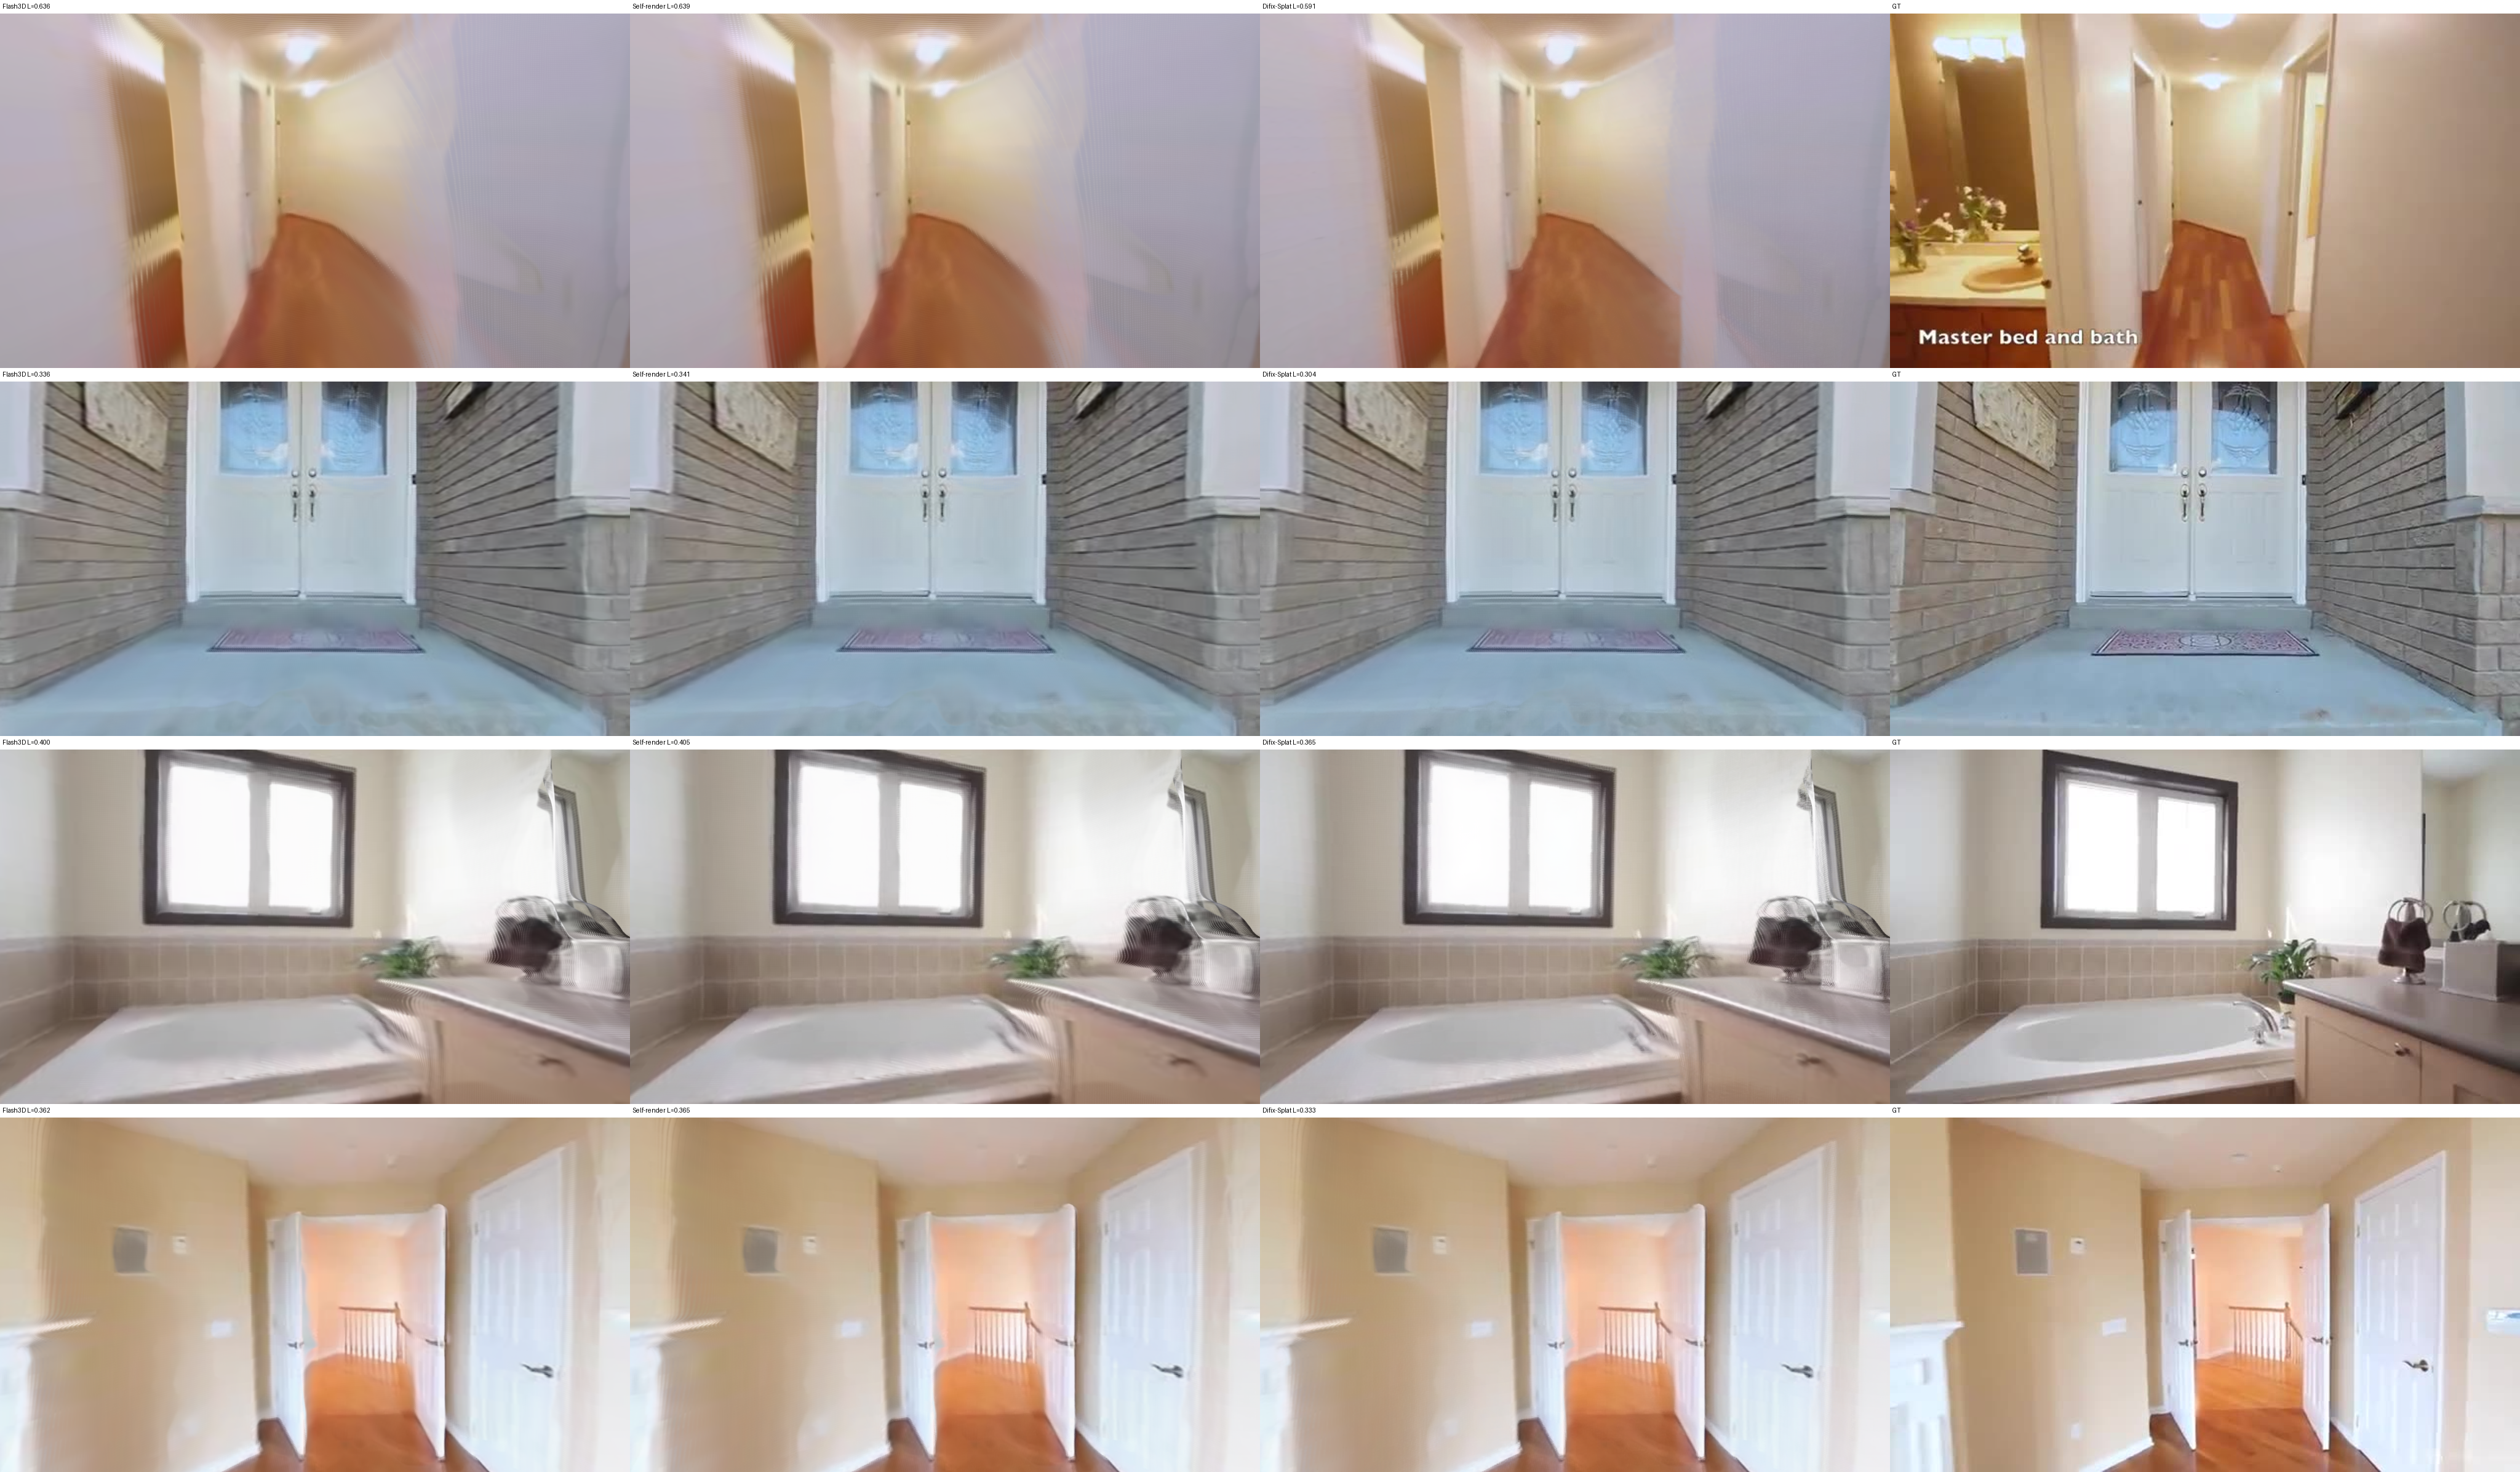
\includegraphics[width=\textwidth]{qualitative.png}
\caption{Large-baseline novel views (rows) under, left to right:
Flash3D baseline, self-render optimization, \method{} (source-referenced Difix
supervision), and ground truth. Per-cell VGG-LPIPS is annotated. \method{}
reduces ghosting and over-smoothing in disoccluded regions; gains are perceptual
and modest, matching the quantitative controls.}
\label{fig:qual}
\end{figure*}

\section{Discussion and Limitations}
\label{sec:discussion}

\method{} shows that the two generative supervisors for feed-forward single-view
Gaussians are complementary---image restoration for perceptual fidelity, video
diffusion for geometric consistency---and that a simple distance-adaptive fusion
captures both, improving every metric at every baseline over Flash3D. Because
most auxiliary views are near the source, the pipeline remains dominated by the
cheap single-step restorer and only invokes the heavier video generator where it
helps (large baselines).

\paragraph{Limitations.}
The 158-sample subset is selected to contain large-baseline targets and is not
the full 3204-frame split; absolute numbers are not directly comparable to
full-split reports. The fusion is a fixed distance schedule; we tried a
per-pixel content-adaptive alternative (Sec.~\ref{sec:contentablation}) and
found it degrades perceptual quality through boundary seams, so a
\emph{learned} whole-frame blend that stays seam-free is the more promising
extension. Gains, while consistent across metrics and datasets, are modest in
magnitude.

\bibliographystyle{plain}
\begin{thebibliography}{99}
\bibitem{flash3d} Szymanowicz et al. Flash3D: Feed-Forward Generalisable 3D Scene Reconstruction from a Single Image. arXiv:2406.04343.
\bibitem{difix} Wu et al. Difix3D+: Improving 3D Reconstructions with Single-Step Diffusion Models. CVPR 2025.
\bibitem{scenesplatter} Zhang et al. Scene Splatter: Momentum 3D Scene Generation from Single Image with Video Diffusion Model. CVPR 2025.
\bibitem{viewcrafter} Yu et al. ViewCrafter: Taming Video Diffusion Models for High-fidelity Novel View Synthesis. arXiv:2409.02048.
\bibitem{mine} Li et al. MINE: Towards Continuous Depth MPI with NeRF for Novel View Synthesis. ICCV 2021.
\bibitem{lpips} Zhang et al. The Unreasonable Effectiveness of Deep Features as a Perceptual Metric. CVPR 2018.
\bibitem{splatterimage} Szymanowicz et al. Splatter Image: Ultra-Fast Single-View 3D Reconstruction. CVPR 2024.
\bibitem{pixelsplat} Charatan et al. pixelSplat. CVPR 2024.
\bibitem{mvsplat} Chen et al. MVSplat. ECCV 2024.
\bibitem{depthsplat} Xu et al. DepthSplat. CVPR 2025.
\bibitem{catsplat} Yang et al. CATSplat. ICCV 2025.
\bibitem{gsenhancer} Liu et al. 3DGS-Enhancer. NeurIPS 2024.
\bibitem{reconfusion} Wu et al. ReconFusion. CVPR 2024.
\bibitem{cat3d} Gao et al. CAT3D. NeurIPS 2024.
\bibitem{deceptivenerf} Liu et al. Deceptive-NeRF/3DGS. ECCV 2024.
\bibitem{acid} Liu et al. Infinite Nature: Perpetual View Generation of Natural Scenes from a Single Image. ICCV 2021.
\end{thebibliography}

\end{document}
